\documentclass[12pt]{beamer}
%\documentclass[20pt,handout]{beamer}
\usetheme{Darmstadt}
\usepackage{graphicx}
%\usepackage[german]{babel}
\usepackage{ngerman}
\usepackage[T1]{fontenc}
\usepackage[utf8]{inputenc}
\usepackage{tikz}
\setbeamertemplate{footline}[frame number]

\newcommand{\cc}[1]{\includegraphics[height=4mm]{img/#1.png}\hspace{1mm}}
\usepackage{ifthen}
\newcommand{\license}[2][]{\\#2\ifthenelse{\equal{#1}{}}{}{\\\scriptsize\url{#1}}}
\usepackage{textcomp}
\usepackage{hyperref}

\pgfdeclareimage[height=.6cm]{c3d2logo}{./img/c3d2.pdf} 


\pgfdeclarelayer{foreground}
\pgfsetlayers{main,foreground}
\logo{\pgfputat{\pgfxy(-1,0)}{\pgfbox[center,base]{\pgfuseimage{c3d2logo}}}}


\title{NSA, Prism und co - Wie schützt man sich vor Überwachung?}
\author{\small Marius Melzer\\\large Chaos Computer Club Dresden}
\date{23.04.2014}

\begin{document}
\maketitle

\section{CCC}
\subsection{}

\begin{frame}
  \frametitle{Chaos Computer Club}
  \begin{figure}
    
\includegraphics[height=0.7\textheight]{img/fingerabdruck.jpg}
  \end{figure}
\end{frame}

\begin{frame}
  \frametitle{Chaos Computer Club}
  \begin{figure}
    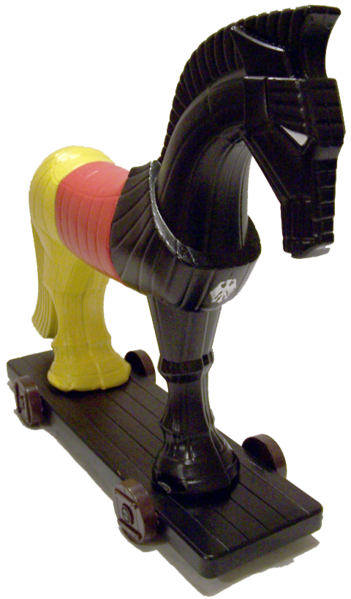
\includegraphics[height=0.7\textheight]{img/trojaner.png}
  \end{figure}
\end{frame}

\begin{frame}
    \frametitle{Chaos Computer Club}
    \begin{itemize}
      \item<1-> Chaos Computer Club Dresden (\url{http://c3d2.de})
          \note{}
      \item<2-> Datenspuren: 13./14.09.2014 \url{http://datenspuren.de}
      \item<3-> Podcasts (\url{http://pentamedia.de})
      \item<4-> Chaos macht Schule
    \end{itemize}
\end{frame}

\section{Datenschutz}
\subsection{}

%% Snowden-Folie

\begin{frame}
    \frametitle{Tempora}
    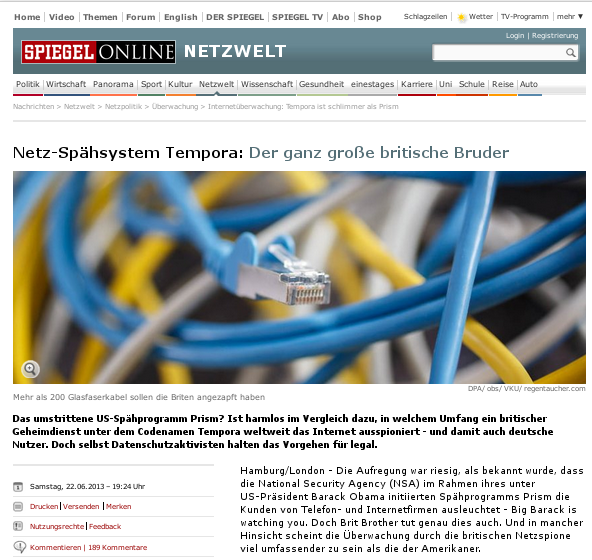
\includegraphics[height=0.7\textheight]{img/spiegel-tempora.png}
\end{frame}

\begin{frame}
    \frametitle{Prism}
    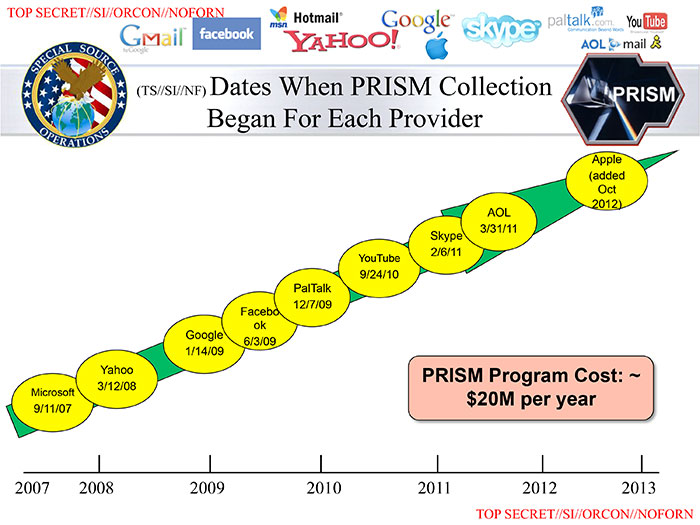
\includegraphics[height=0.7\textheight]{img/prism.jpg}
\end{frame}

%% http://www.theconnectivist.com/2013/06/the-expanding-consolidation-of-the-consumer-internet/

%% Angry Birds-Folie

\begin{frame}
    \frametitle{Bundespräsident Gauck zur NSA-Überwachung}
    \begin{center}
      "`Wir wissen z.B., dass es nicht so ist, wie bei der Stasi und dem KGB, dass es dicke Aktenbände gibt, wo unsere Gesprächsinhalte alle aufgeschrieben und schön abgeheftet sind. Das ist es nicht."'
      \end{center}
\end{frame}

\begin{frame}
    \frametitle{Stasi vs. NSA}
    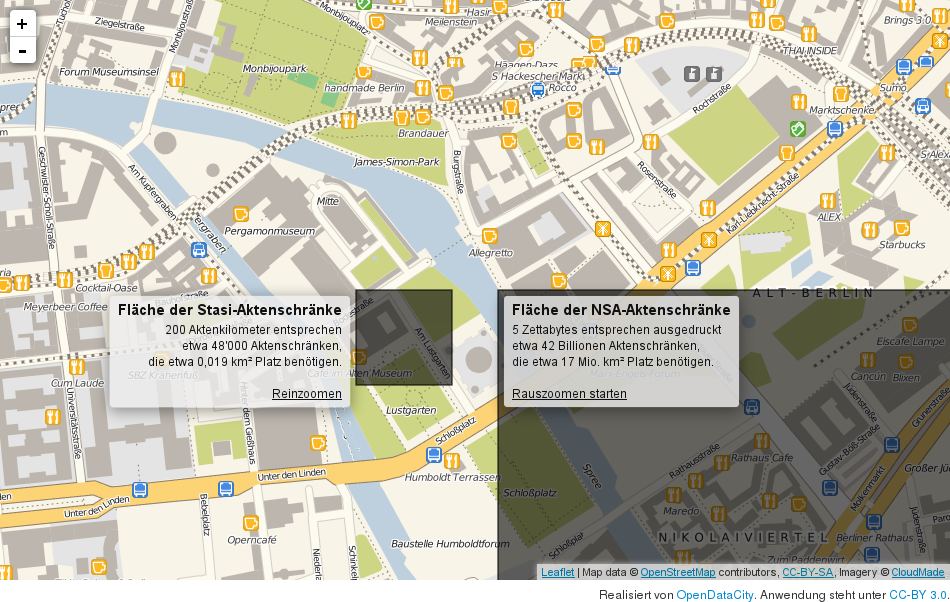
\includegraphics[height=0.7\textheight]{img/akten1.png}
\end{frame}

\begin{frame}
    \frametitle{Stasi vs. NSA}
    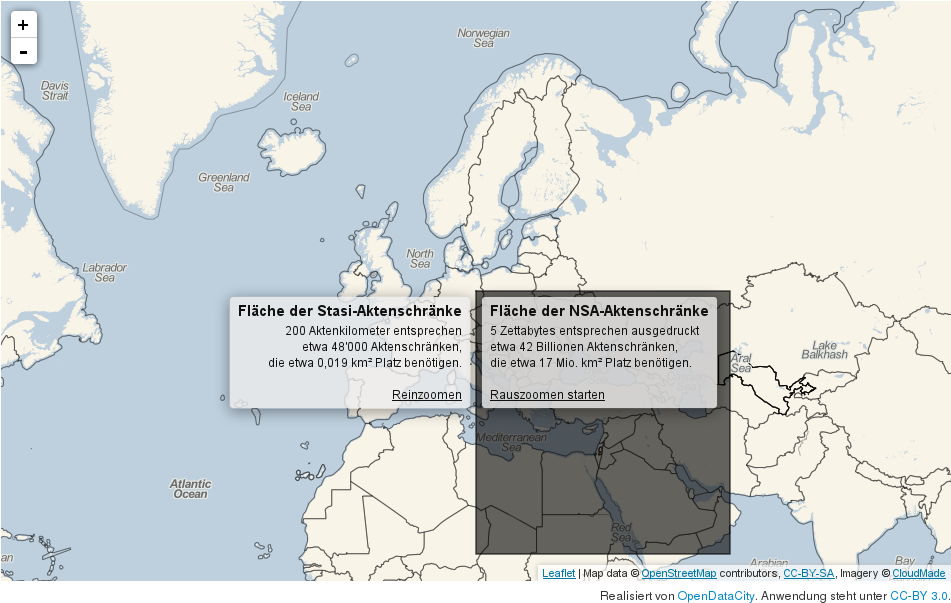
\includegraphics[height=0.7\textheight]{img/akten2.png}
\end{frame}

\begin{frame}
    \frametitle{Merkels Handy}
    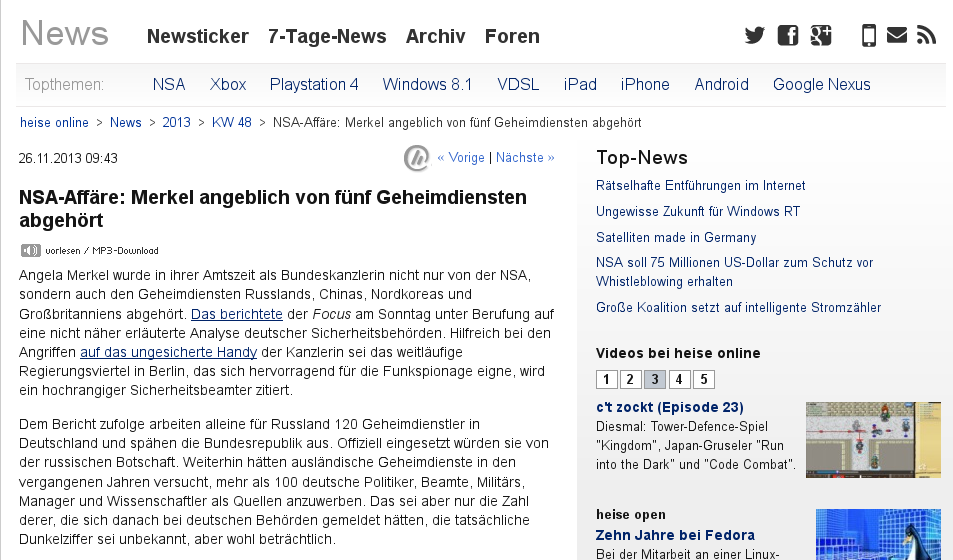
\includegraphics[height=0.7\textheight]{img/heise-merkel.png}
\end{frame}

\section{Metadaten}
\subsection{}

\begin{frame}
  \frametitle{Vorratsdatenspeicherung (USA)}
    \begin{center}
      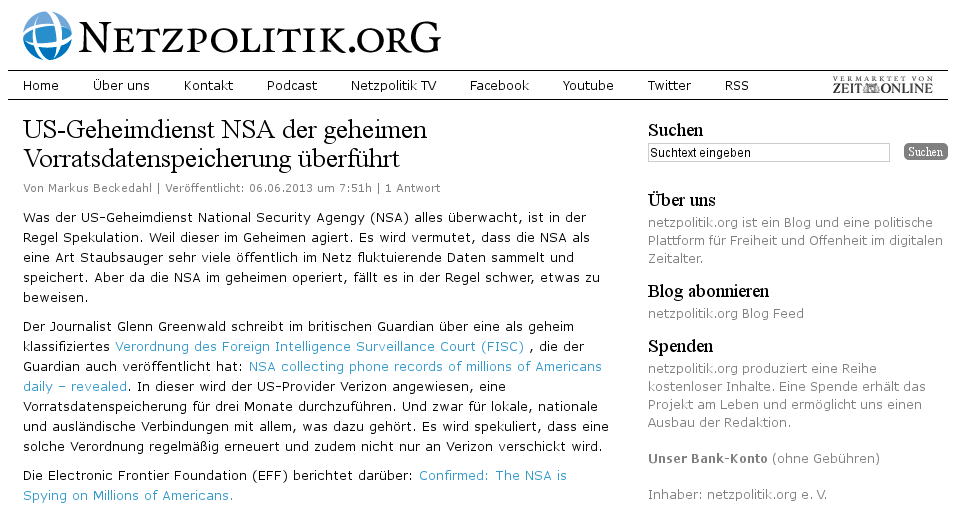
\includegraphics[height=5cm]{img/netzpolitik-verizon.png}
    \end{center}
\end{frame}

\begin{frame}
  \frametitle{Vorratsdatenspeicherung (Deutschland)}
    \begin{center}
      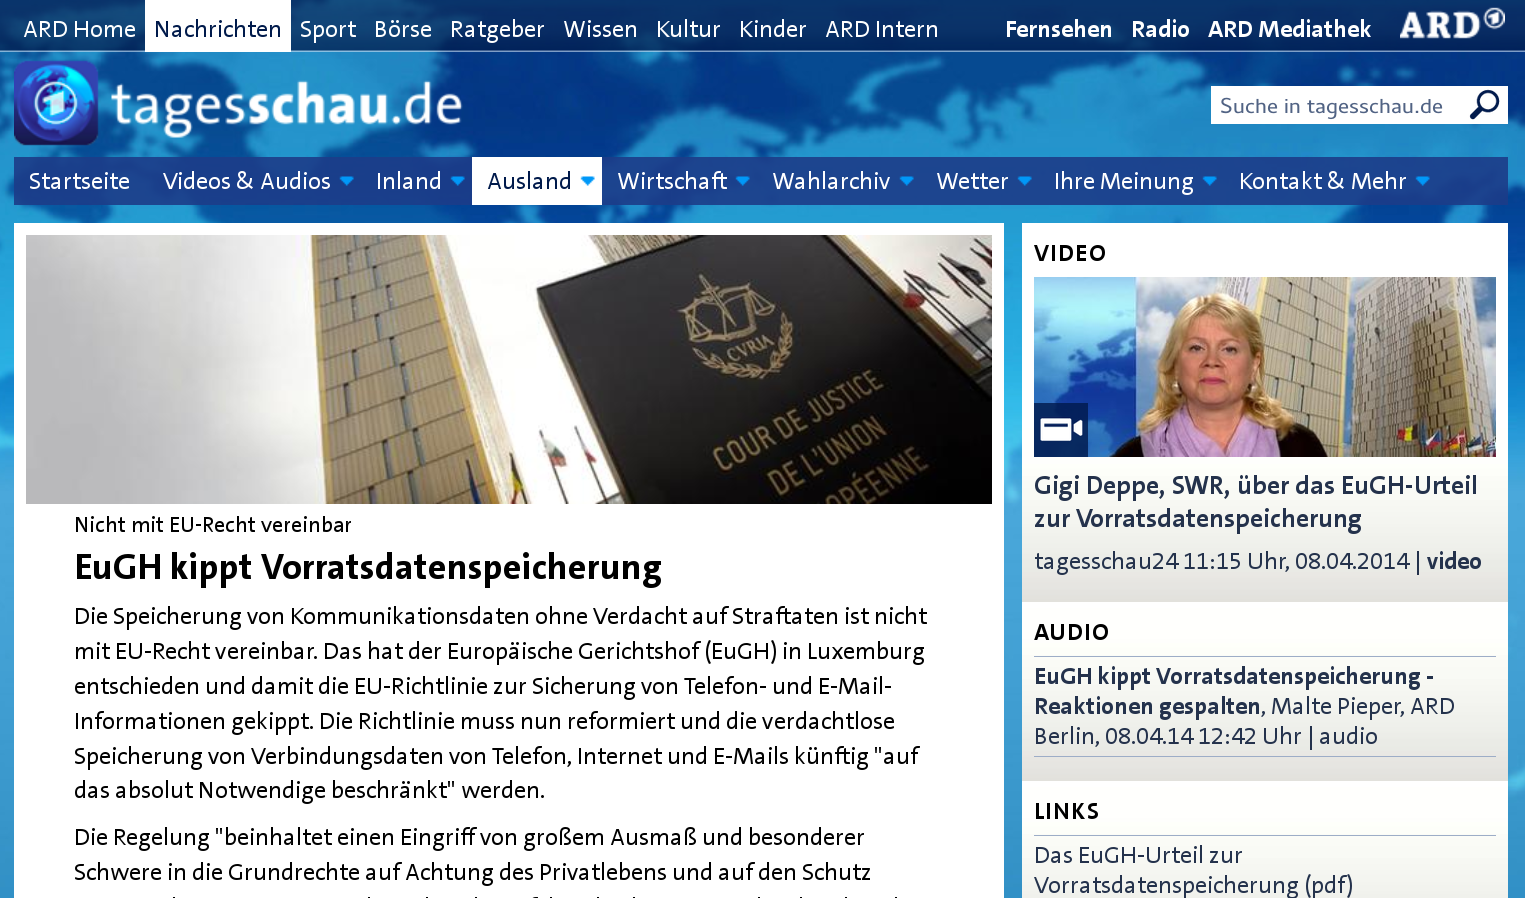
\includegraphics[height=5cm]{img/tagesschau-vds.png}
    \end{center}
\end{frame}

\begin{frame}
  \frametitle{Metadaten}
    \begin{center}
      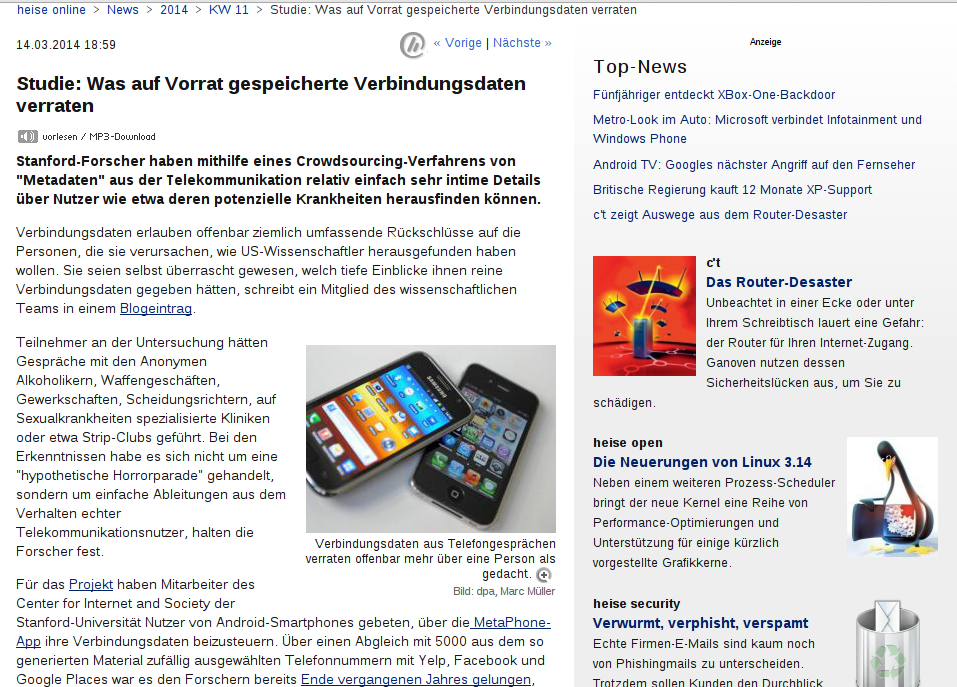
\includegraphics[height=5cm]{img/metadaten_studie.png}
    \end{center}
\end{frame}

\begin{frame}
    \frametitle{Metadaten}
    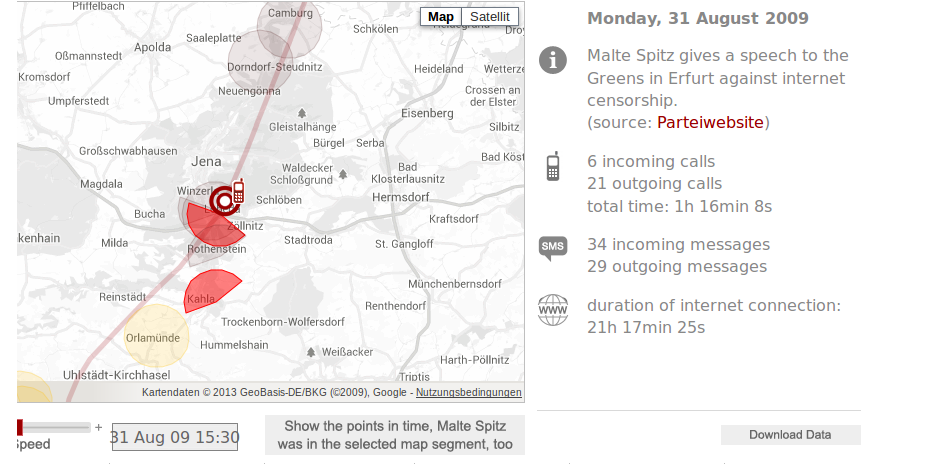
\includegraphics[height=0.7\textheight]{img/maltespitz.png}
\end{frame}

\begin{frame}
    \frametitle{Metadaten - Lightbeam}
    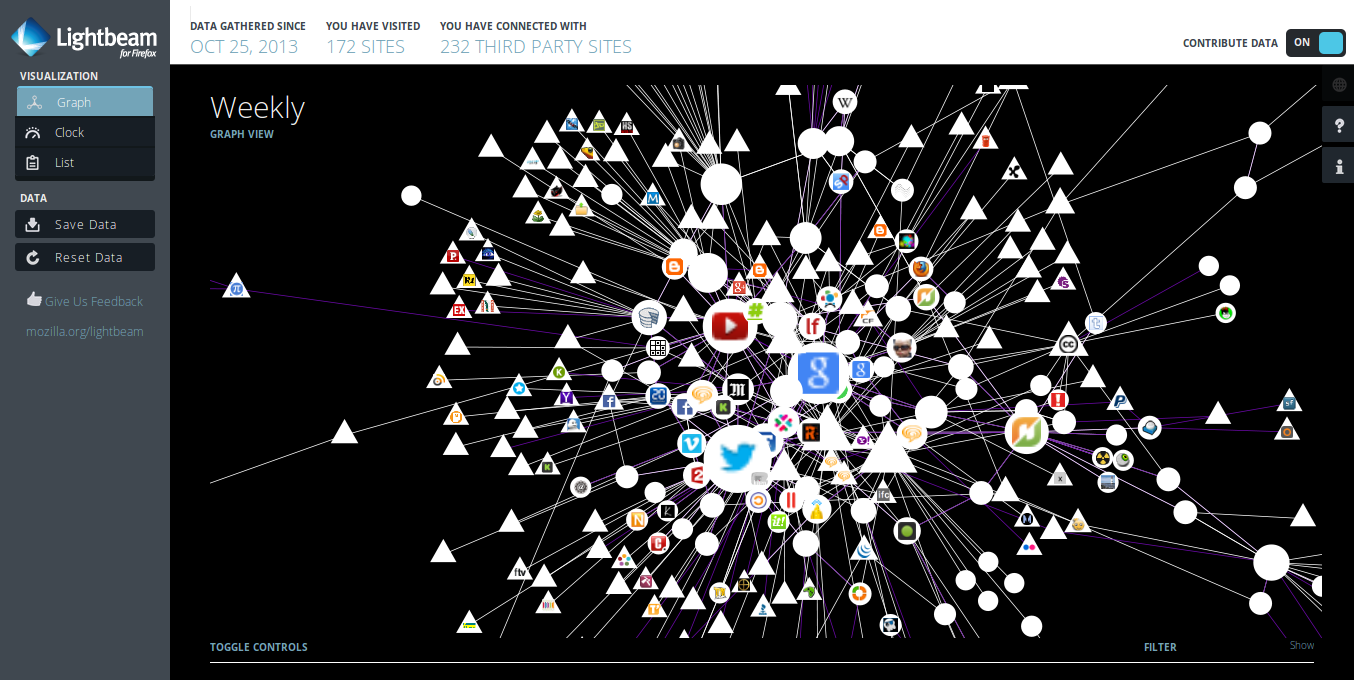
\includegraphics[height=0.7\textheight]{img/lightbeam.png}
  \\{\small \href{http://www.flickr.com/photos/8517757@N03/10538205035/in/photolist-h4e4dg}{Grafik:} \href{http://creativecommons.org/licenses/by-sa/3.0/deed.en}{\cc{by-sa}} Clint Lalonde}
\end{frame}

\begin{frame}
    \frametitle{Tor}
    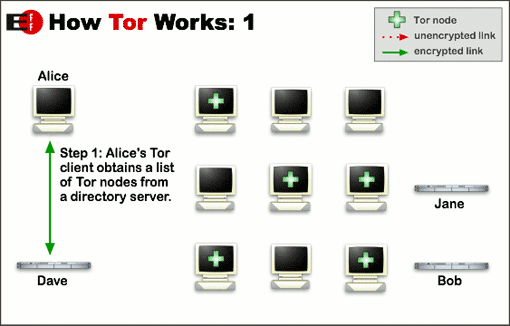
\includegraphics[height=0.7\textheight]{img/tor1.png}
    \\{\small \href{https://www.torproject.org/images/htw1.png}{Grafik}: \href{https://creativecommons.org/licenses/by/3.0/us/}{\cc{by}} The Tor Project}
\end{frame}

\begin{frame}
    \frametitle{Tor}
    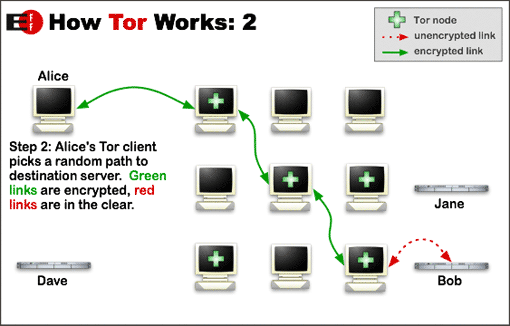
\includegraphics[height=0.7\textheight]{img/tor2.png}
    \\{\small \href{https://www.torproject.org/images/htw2.png}{Grafik}: \href{https://creativecommons.org/licenses/by/3.0/us/}{\cc{by}} The Tor Project}
\end{frame}

\begin{frame}
    \frametitle{Tor}
    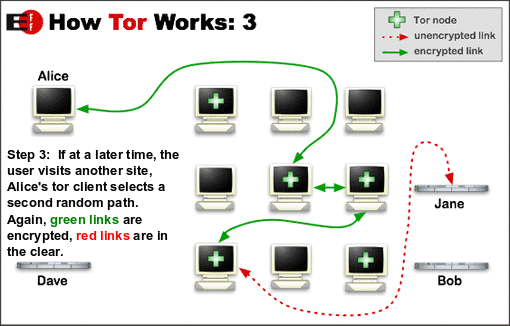
\includegraphics[height=0.7\textheight]{img/tor3.png}
    \\{\small \href{https://www.torproject.org/images/htw3.png}{Grafik}: \href{https://creativecommons.org/licenses/by/3.0/us/}{\cc{by}} The Tor Project}
\end{frame}

\begin{frame}
  \frametitle{Tor}
  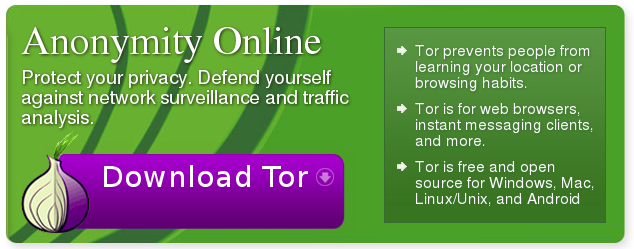
\includegraphics[height=0.5\textheight]{img/tor-banner.png}
\end{frame}

\begin{frame}
    \frametitle{Zensur}
    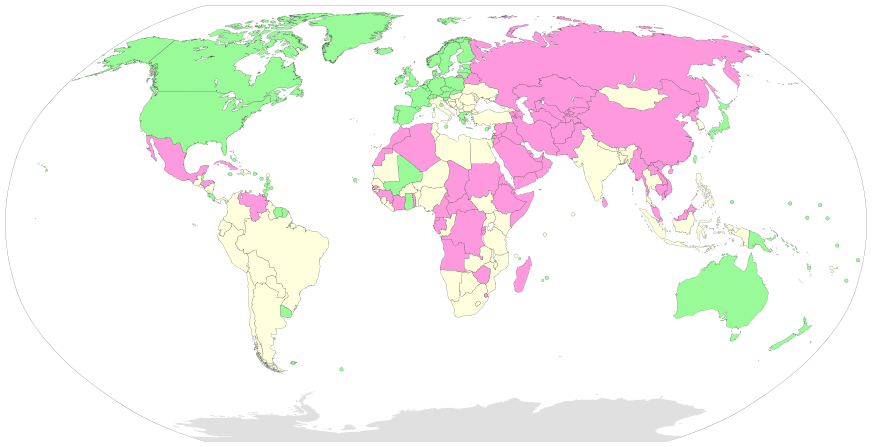
\includegraphics[height=0.7\textheight]{img/zensur.png}
    \\{\small \href{http://upload.wikimedia.org/wikipedia/commons/5/51/RWB-PressFreedomIndex2013-WorldMap.svg}{Grafik}: \href{http://creativecommons.org/licenses/by-sa/3.0/deed.en}{\cc{by-sa}} Jeff Ogden (W163)}
\end{frame}

\begin{frame}
    \frametitle{Tor in der Türkei}
    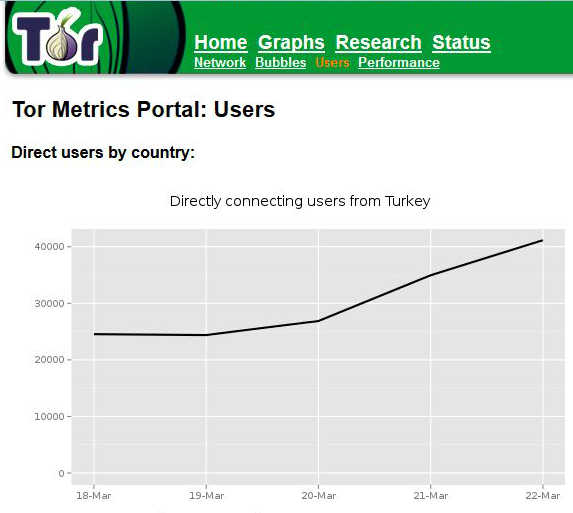
\includegraphics[height=0.7\textheight]{img/tor-tuerkei.jpg}
\end{frame}

\begin{frame}
    \frametitle{Anonymität unter Vollüberwachung}
    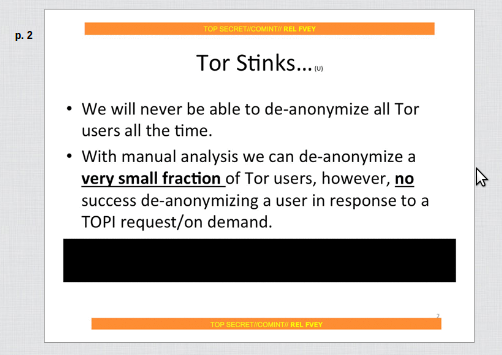
\includegraphics[height=0.7\textheight]{img/torstinks.png}
\end{frame}

\section{Inhalte}
\subsection{}

\begin{frame}
    \frametitle{Verschlüsselung: Analogie}
    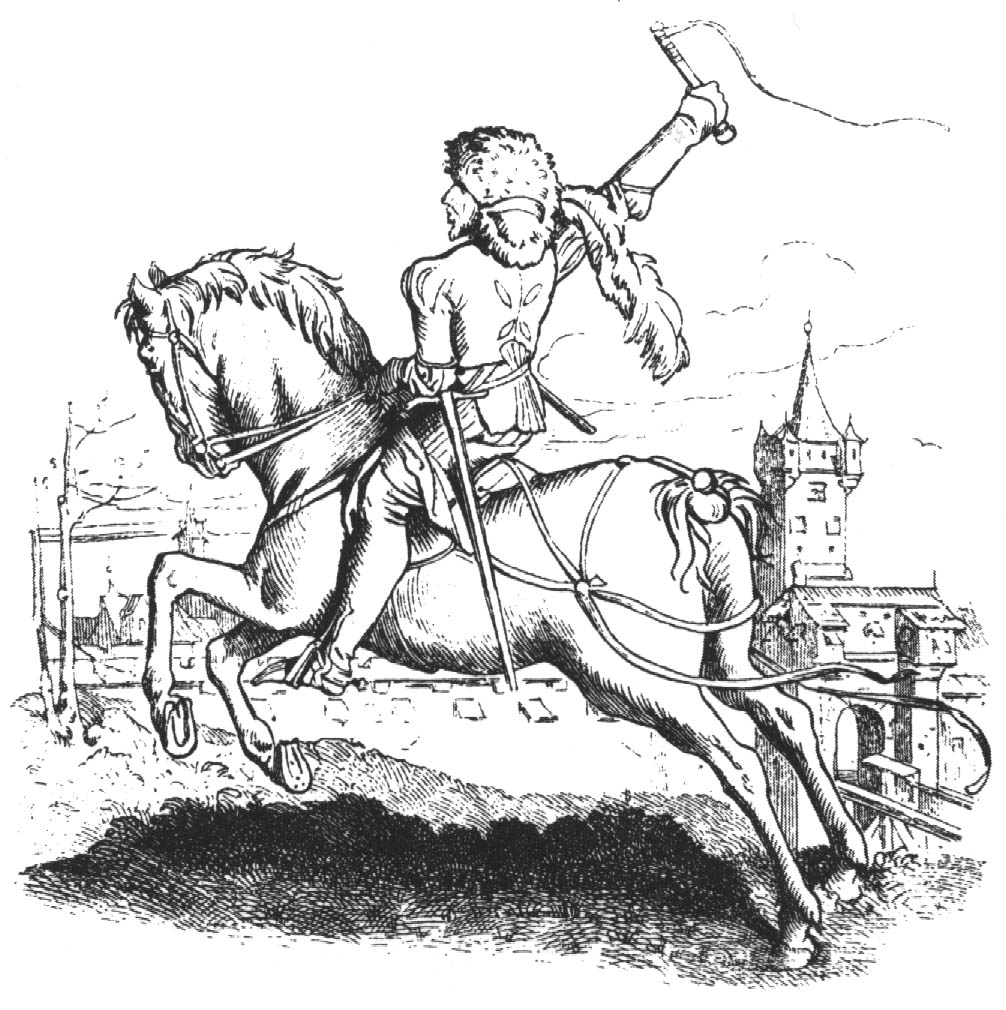
\includegraphics[height=0.7\textheight]{img/bote.jpg}
    {\\ \small \href{http://commons.wikimedia.org/wiki/File:Reitbote.jpg}{Grafik}: \href{http://creativecommons.org/licenses/by-sa/2.5/deed.en}{\cc{by-sa}} Ronald Preuss}
\end{frame}

\begin{frame}
    \frametitle{Verschlüsselung: Asymmetrische}
    \includegraphics[height=0.7\textheight]<2->{img/asym_encryption.png}
\end{frame}

\begin{frame}
    \frametitle{SSL / TLS}
    \begin{itemize}
      \item<2-> SSL = Secure Socket Layer
      \item<3-> eingesetzt im Web, Mail, ...
    \end{itemize}
\end{frame}

\begin{frame}
    \frametitle{SSL im Browser}
    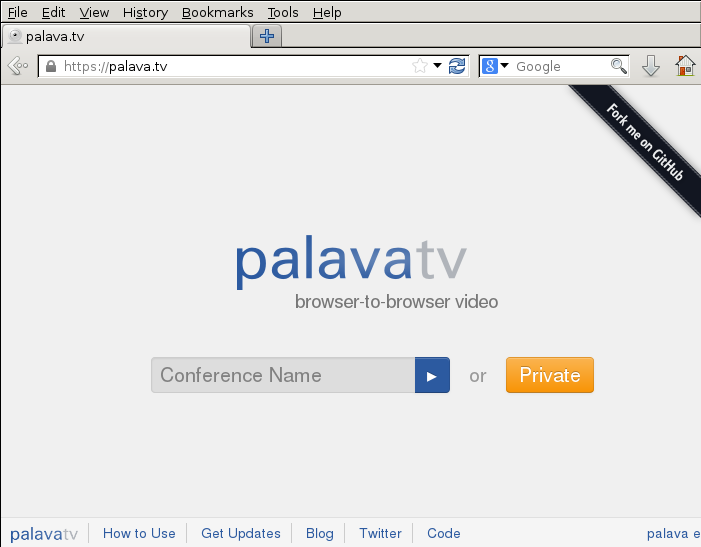
\includegraphics[height=0.7\textheight]{img/ssl_verified.png}
\end{frame}

\begin{frame}
    \frametitle{SSL im Browser}
    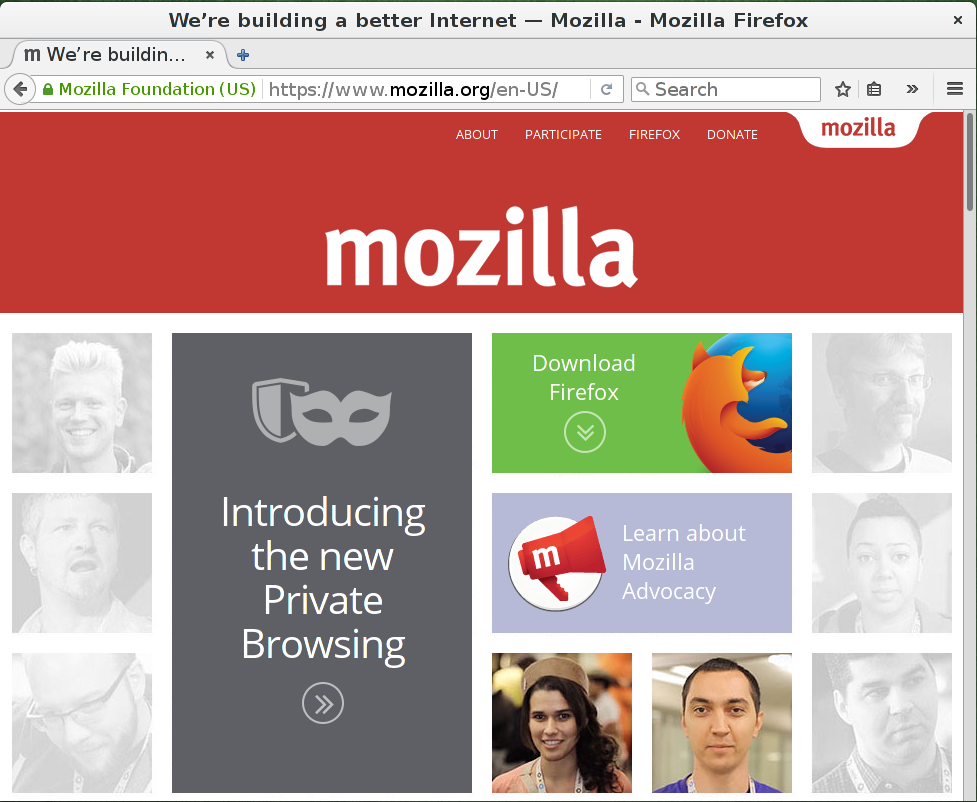
\includegraphics[height=0.7\textheight]{img/ssl_special.png}
\end{frame}

\begin{frame}
    \frametitle{SSL im Browser}
    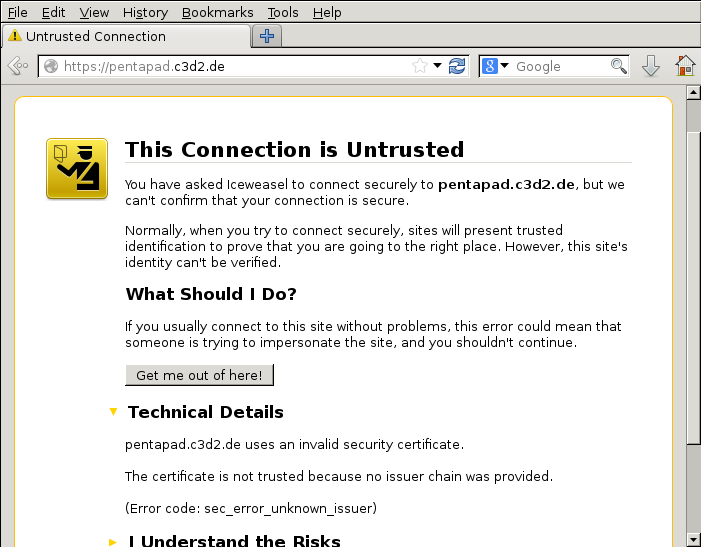
\includegraphics[height=0.7\textheight]{img/ssl_unverified.png}
\end{frame}

\begin{frame}
    \frametitle{Zertifizierungsstellen}
    \begin{center}
      \includegraphics[height=5cm]<2->{img/zertifikate.png}
    \end{center}
\end{frame}

\begin{frame}
  \frametitle{HTTPS Everywhere}
    \begin{center}
      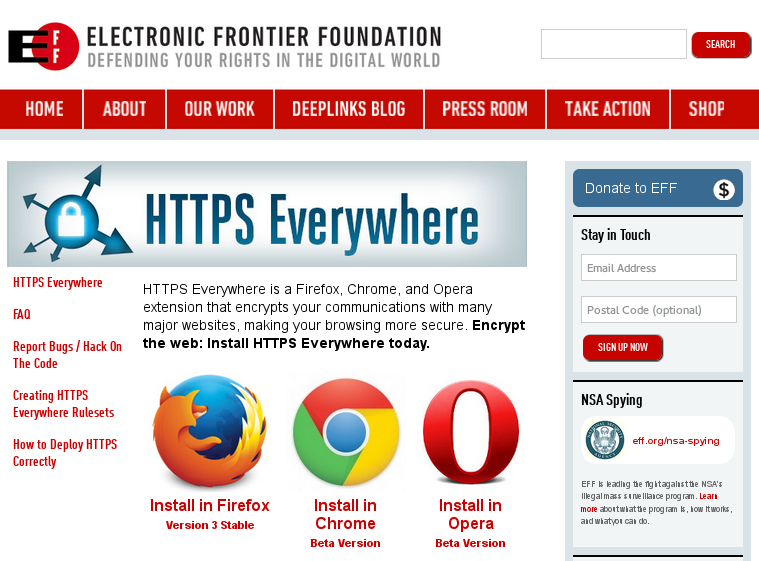
\includegraphics[height=5cm]{img/https-everywhere.png}
    \end{center}
\end{frame}

\begin{frame}
   \frametitle{E-Mail Verschlüsselung}
   \vspace{-1cm}
   \begin{center}
      
\includegraphics[width=0.5\textwidth]{img/Gnupg_logo}
   \end{center}
   \begin{itemize}
      \item GNU Privacy Guard
      \item Verschlüsselungssoftware für Texte und Dateien
      \item Windows: \textbf{GPG4Win - \texttt{http://www.gpg4win.org/}}
      \item Mac OS X: \textbf{MacGPG - \texttt{https://gpgtools.org/}}
      \item Android: \textbf{APG}
   \end{itemize}
\end{frame}

\begin{frame}
   \frametitle{E-Mail Verschlüsselung auf dem PC}
   \begin{columns}[T]
      \column{5cm}
      \textbf{\Large{}Mozilla Thunderbird mit Enigmail-Plugin}{\Large \par}
      \column{2cm}
      
\includegraphics[width=1\textwidth]{img/Mozilla_Thunderbird_3}
   \end{columns}
\end{frame}

\begin{frame}
   \frametitle{E-Mail Verschlüsselung auf dem PC}
   \begin{columns}[T]
      \column{5cm}
      \begin{center}
              \textbf{\Large{}Mozilla Firefox mit Mailvelope-Plugin}{\Large \par}
     \end{center}
      \column{2cm}
      
\includegraphics[width=0.8\textwidth]{img/502400-64}
         \vspace{1cm}
         
\includegraphics[width=2cm]{img/Beta-badge}
    \end{columns}
\end{frame}

\begin{frame}
  \frametitle{Ende-zu-Ende-Verschlüsselung II}
  \begin{itemize}
    \item<2-> OTR für Jabber:
      \begin{itemize}
        \item Pidgin mit OTR-Plugin für Linux und Windows
        \item GibberBot oder Xabber für Android
        \item Adium für Mac, ChatSecure für iOS
      \end{itemize}
    \item<3-> palava.tv für Videotelefonie
    \item<4-> Redphone für Handytelefonate (Android)
    \item<5-> TextSecure für Nachrichten (Android)
  \end{itemize}
\end{frame}

\begin{frame}
  \frametitle{Authentifizierung}
    \begin{center}
      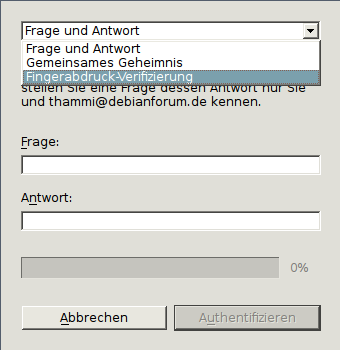
\includegraphics[height=5cm]{img/auth.png}
    \end{center}
\end{frame}

\begin{frame}
  \frametitle{TextSecure}
    \begin{center}
      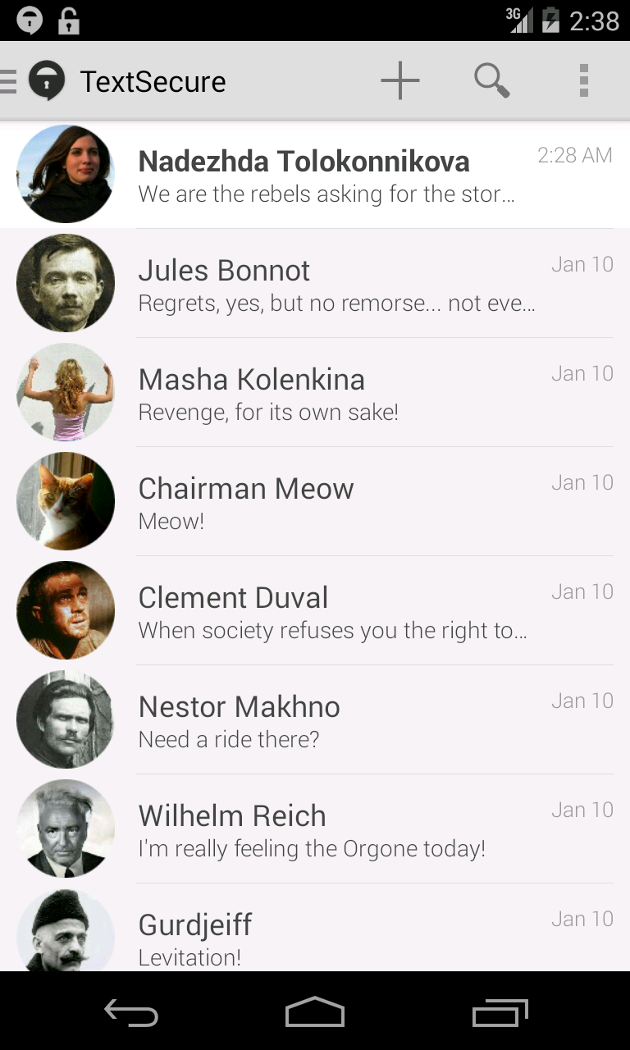
\includegraphics[height=6cm]{img/textsecure1.png}
      \hspace{0.5cm}
      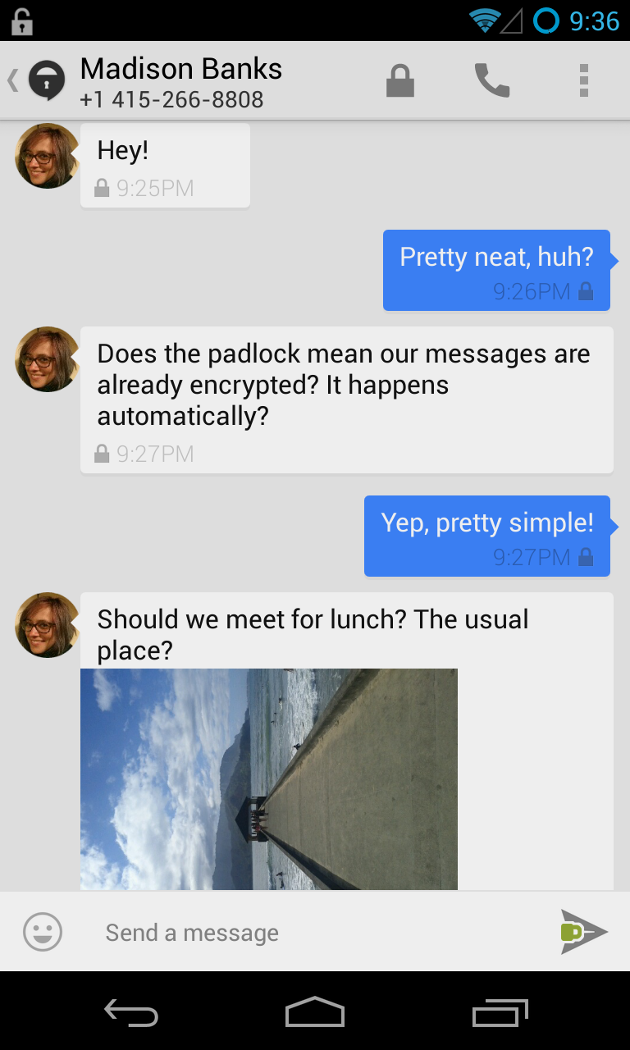
\includegraphics[height=6cm]{img/textsecure2.png}
    \end{center}
\end{frame}
 
\begin{frame}
  \frametitle{Diskussion}
  \begin{center}
    {\Large Diskussion}\\
    \vspace{5mm} 
    \href{https://github.com/c3d2/cms-nsa}{Folien}: \href{https://creativecommons.org/licenses/by-sa/4.0/}{\cc{by-sa}} Chaos Computer Club Dresden \\
    \vspace{4mm}
    Twitter: @faraoso, Email und Jabber: marius@rasumi.net\\GPG-Fingerprint: 52DEFC3E\\
    \vspace{4mm}
    CMS Dresden: schule@c3d2.de
  \end{center}
\end{frame}

\end{document}
